\section{FEFF9 Design}

FEFF is an \textit{ab initio} absorption simulation software based on real-space multiple scattering (RSMS) and the Greene's function. The current version, FEFF9, calculates a self-consistent density function over a wide range of structures by considering the excited state properties within an
all-electron framework \cite{feff-new-dev}. 

Like other density-functional theory (DFT) software, FEFF begins with an initial guess for the electronic density. Then, using an optimization algorithm like gradient descent (See \ref{sec:optimizers}), FEFF iterates through a series of calculations until the resulting potential matches the initial potential (self-consistency). This process is depicted in Figure \ref{fig:feff-dft-diagram}.

\begin{figure}
    \centering
    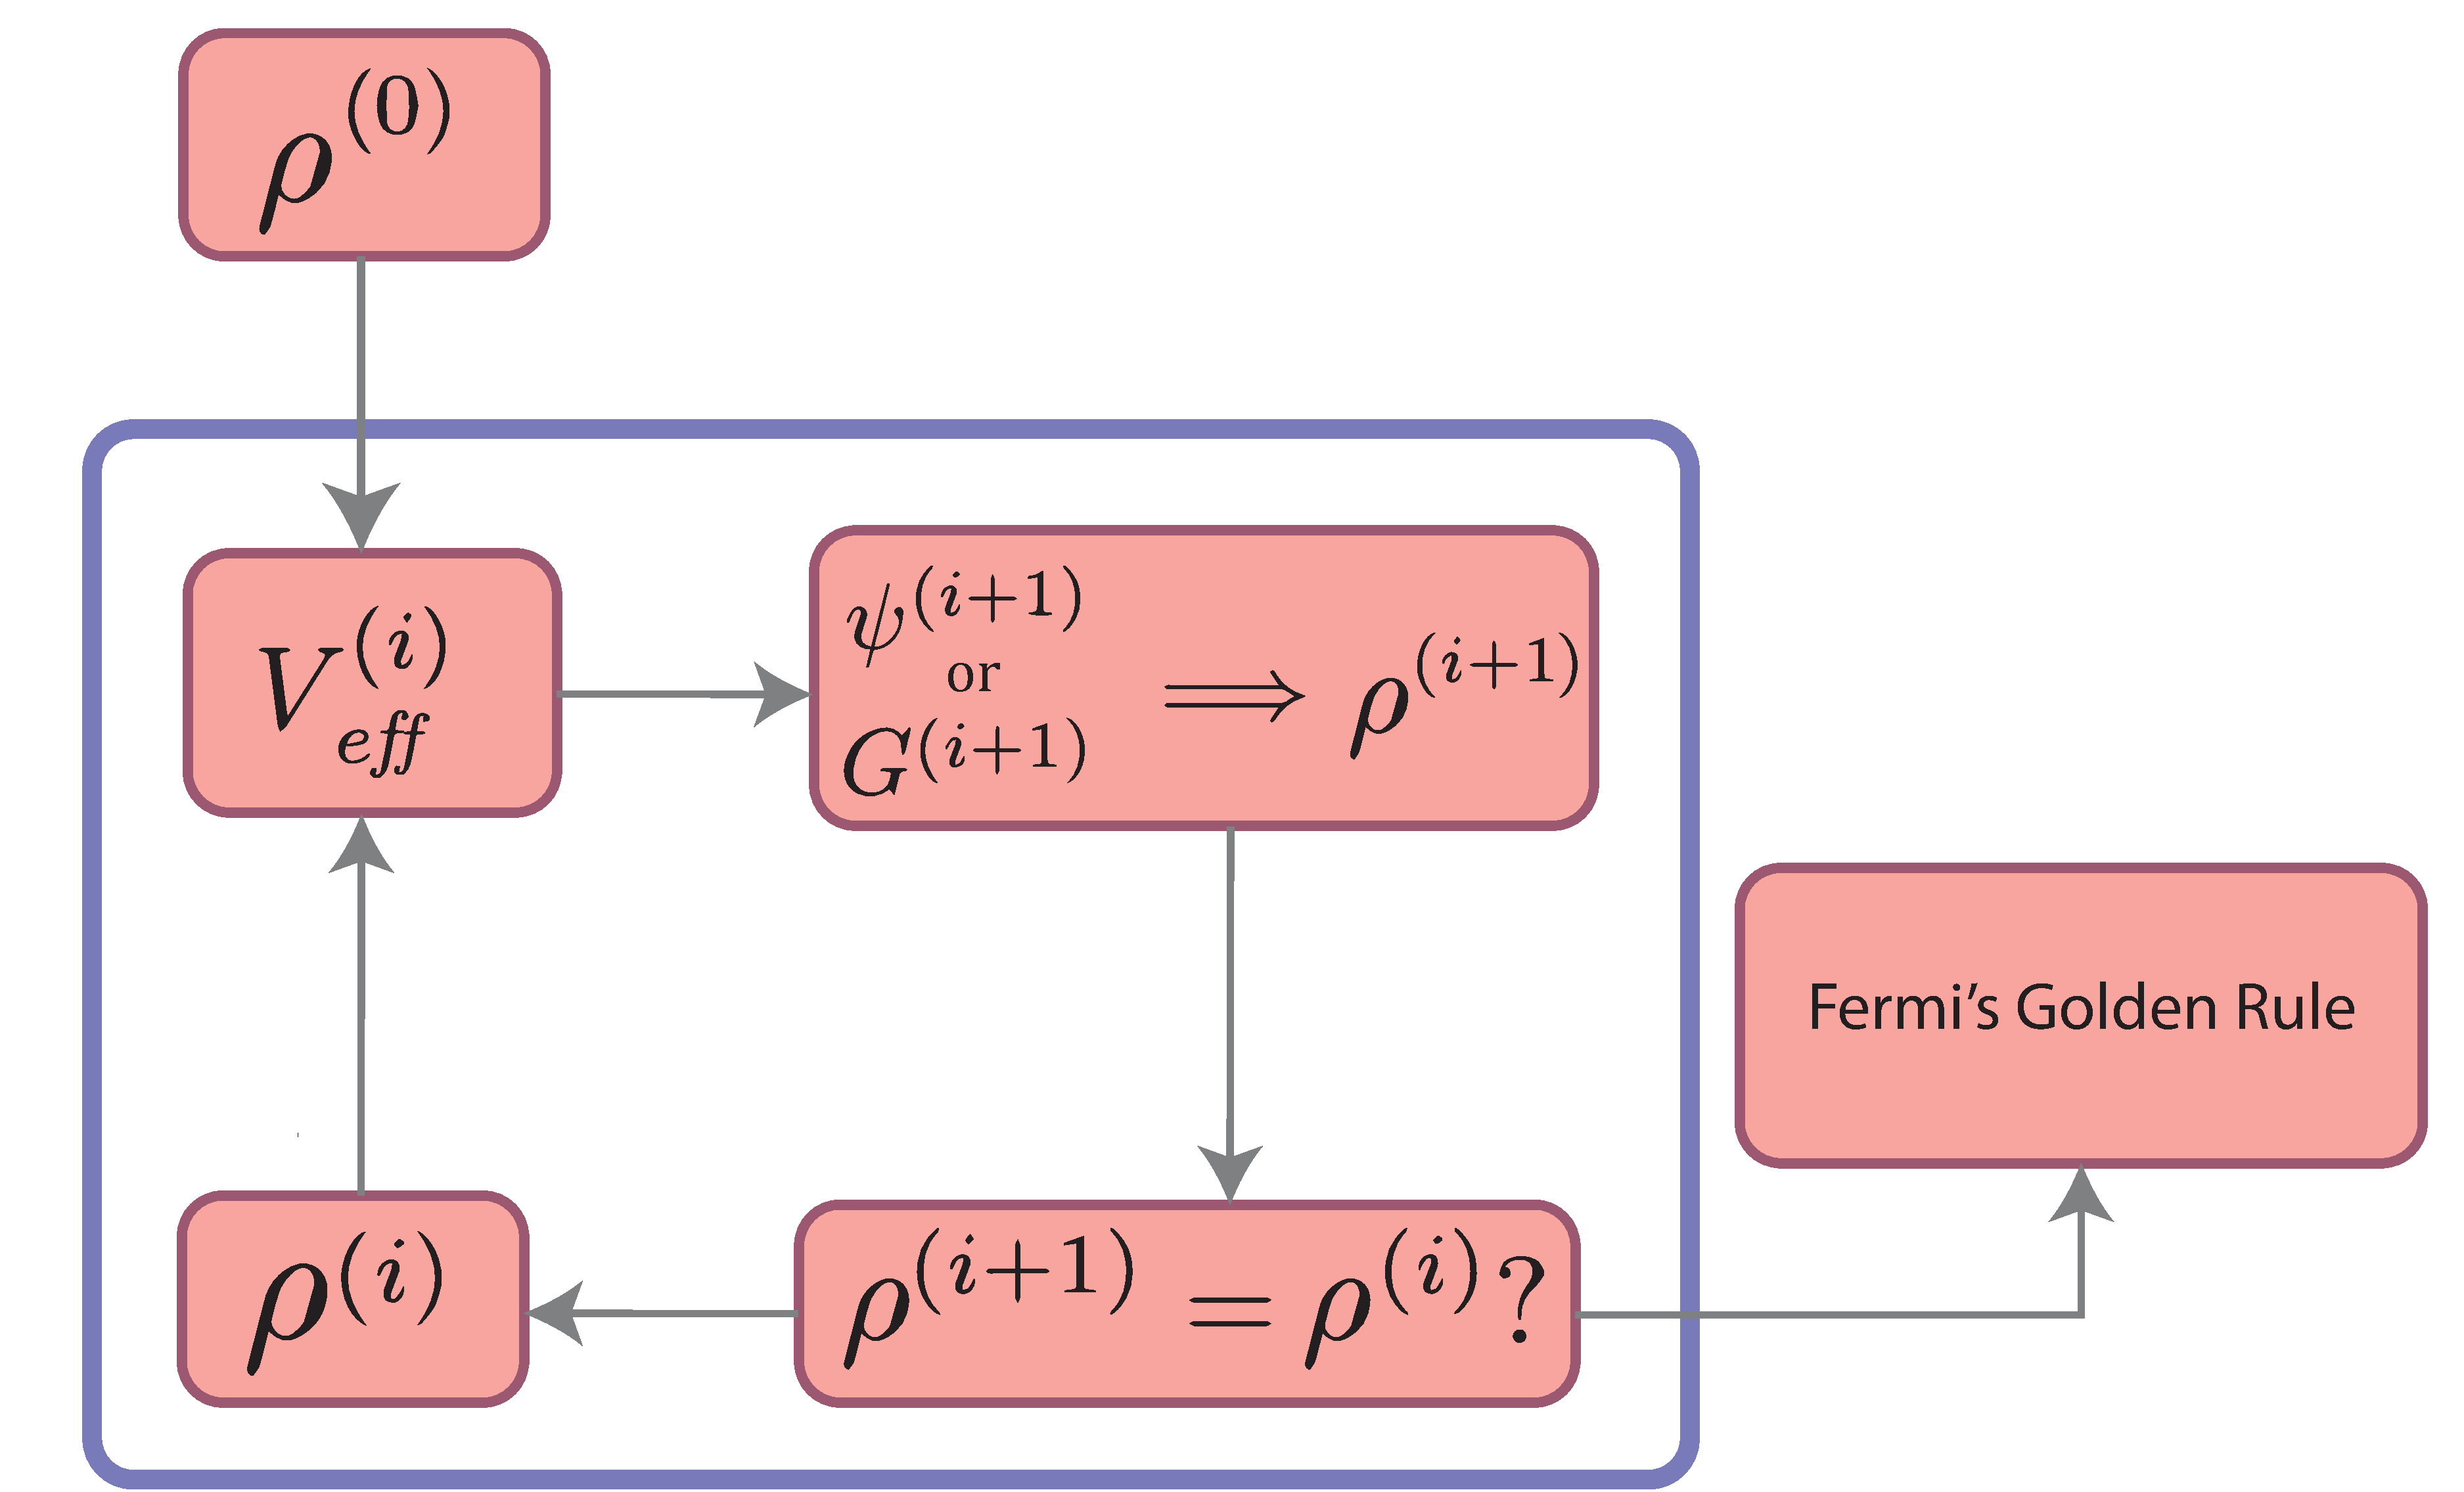
\includegraphics[width=\linewidth]{Chapters/Figures/dft-feff-diagram.pdf}
    \caption[FEFF Diagram]{Feff Diagram works by ...}
    \label{fig:feff-dft-diagram}
\end{figure}

FEFF first makes an initial guess for the electronic density, then calculates the initial potential---which is a functional of that density. Using this potential and the Schrodinger equation, FEFF calculates Green's function \cite{greens-function-xafs-2021}. Finally, using Green's function, FEFF checks if the potential is self-consistent. If not, the potential is updated, and the iterative process repeats. Using Green's function, FEFF calculates the wave function and the absorption spectrum \cite{feff-citation} \cite{rehr2010parameter}. The exact mathematical formalism is beyond the scope of this thesis.

\section{Green's Function}

% that includes inelastic losses, self-energy effects, and vibrational
% damping.

% https://iopscience.iop.org/article/10.1088/1742-6596/430/1/012001/pdf  and that lecture on FEFF
